\chapter{Introducing 3D Data Processing}

\section{3D Data Representations}
\begin{itemize}
    \item{
        \emph{Point Cloud Representation}:
        A set of 3D points.
        Raw measurements of many depth cameras.
        Point clouds are unordered and irregular in that there is no specific relation
        between each points. This makes it hard to use operations such as convolutions.
        Point clouds are heterogeneous in that different point clouds may include different
        numbers of points. This makes it hard for efficient batch processing (
        PyTorch3D handles this problem).
    }
    \item{
        \emph{Mesh Representation}:
        A set of vertices (3D points) and faces (polygons).
        Result of post-processing of raw measurements of depth cameras.
        Geometric information is embedded in mesh representations, making networks such
        as graph convolution networks operable on meshes.
        Meshes also have heterogeneous data issues that PyTorch3D handles.
    }
    \item{
        \emph{Voxel Representation}:
        Representation by dividing a 3D cube into voxels (smaller cubes).
        Voxels are ordered and regular, making convolution operations are possible.
        Voxels require more computer memory, methods such as hashing reduces this problem.
    }
    \item{
        \emph{Other Representations}:
        Multi-view representations, RGB-D representations are other methods of
        3D data representations.
    }
\end{itemize}

\section{3D Data File Formats}
\begin{itemize}
    \item{
        \emph{PLY}:
        Data format capable of mesh representation. Can be either in ASCII format
        or binary format. Composed of a header section and a data section.
    }
    \item{
        \emph{OBJ}:
        Data format capable of mesh representation. OBJ files are connected with a MTL
        (Material Template Library) file that defines surface shading properties.
    }
\end{itemize}

\section{3D Coordinate Systems}
\begin{itemize}
    \item{
        \emph{World Coordinate System}:
        World coordinate systems define the origin and axis globally
        and is independent with the object orientation or camera orientation.
    }
    \item{
        \emph{Camera View Coordinate System}:
        Camera view coordinate systems place the origin at the camera projection
        center and the three axes accordingly. PyTorch3D defines the axes to have
        the $x$ axis to the left, $y$ axis to the top, and the $z$ axis to the front.
    }
    \item{
        \emph{NDC System}:
        The NDC (Normalized Device Coordinate) system confines the volume that
        a camera can render. The $x$ and $y$ values range from $-1$ to $1$, while
        the $z$ value range from $z_{near}$ to $z_{far}$. Any object outside these
        bounds do not get rendered.
    }
\end{itemize}

\section{Camera Models}
\begin{itemize}
    \item{ \emph{Perspective Camera Models} }
    \item{ \emph{Orthographic Camera Models} }
\end{itemize}
\begin{figure}[ht]
  \centering
   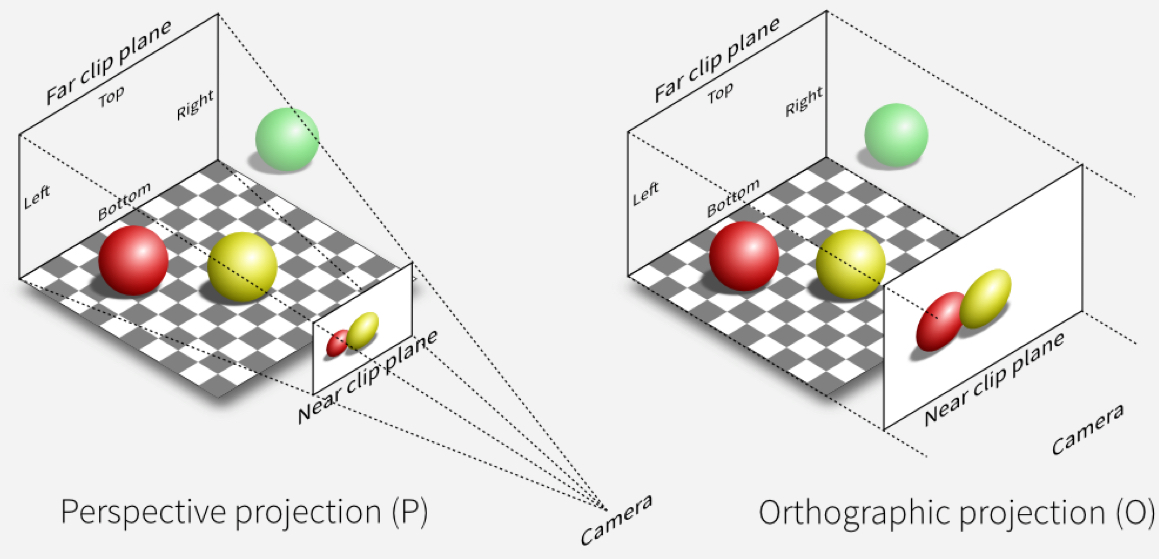
\includegraphics[width=0.8\linewidth]{./figures/ch1-camera-models.jpeg}
   \caption{Difference between perspective camera models and orthographic camera models.}
\end{figure}

